\documentclass{article}

\usepackage[left=2.5cm, right=2.5cm, top=2.5cm, bottom=2.5cm]{geometry}
\usepackage{amsmath}
\usepackage{listings}
\usepackage{color}
\usepackage{placeins}
\usepackage{graphicx}
\graphicspath{ {C:\Users\Dell\Documents\Graduate - Economics\Empirical Industrial Organisation I\pset3_working} }

\title{Empirical Industrial Organisations I: PSet 3}
\author{S M Sajid Al Sanai}
\date{December 4, 2018}

\begin{document}

\maketitle
\pagenumbering{arabic}
\tableofcontents

\lstset{
	frame=lines,
	basicstyle=\small\sffamily,
	tabsize=4,
	columns=fixed,
	showstringspaces=false,
	showtabs=false,
	keepspaces,
	commentstyle=\color{red},
	keywordstyle=\color{blue}
}

\newpage

\section{Question I}

\subsection{Choice-Specific Value Functions}

Define the maximisation problem:

\begin{equation}
\Big( \sum_{t=1} ^{\infty} \beta^t[ u(x_t,i_t,\theta_1) + \epsilon_t(i_t) ] \Big)
\end{equation}

\noindent Define the utility function:

\begin{equation}
  u( x_t, i_t; \theta_1 ) + \epsilon_t( i_t ) =\begin{cases}
    u( x_t, 1; \theta_1 ) + \epsilon_t( 1 ), & \text{if $i_t=1$}.\\
    u( x_t, 0; \theta_1 ) + \epsilon_t( 0 ), & \text{if $i_t=0$}.
  \end{cases}
\end{equation}

\begin{equation}
  u( x_t, i_t; \theta_1 ) + \epsilon_t( i_t ) =\begin{cases}
    -RC - c( 0, \theta_1 ) + \epsilon_t( 1 ), & \text{if $i_t=1$}.\\
    -c( x_t, \theta_1 ) + \epsilon_t( 0 ), & \text{if $i_t=0$}.
  \end{cases}
\end{equation}

\noindent Define the shorthand utility function:

\begin{equation}
\equiv u( x_t, i_t; \theta_1 ) + \epsilon_t( i_t ) = -RC * i_t - c( [ 1 - i_t ] * x_t, \theta_1 ) + \epsilon_t( i_t )
\end{equation}

\noindent Define the value function:

\begin{equation}
V( x_t, \epsilon_t ) = max \{ \tilde{V} ( x_t, \epsilon_t(1), 1 ), \tilde{V} ( x_t, \epsilon_t(0), 0 ) \}
\end{equation}

\noindent Define the choice-specific value functions:

\begin{equation}
  \tilde{V} ( x_t,\epsilon_t( i_t ),  i_t ) =\begin{cases}
    u( x_t, 1; \theta_1 ) + \epsilon_t( 1 ) + \beta E_t V ( 0, \epsilon_{ t+1 } ), & \text{if $i_t=1$}.\\
    u( x_t, 0; \theta_1 ) + \epsilon_t( 0 ) + \beta E_t V ( x_{ t+1 }, \epsilon_{ t+1 } ), & \text{if $i_t=0$}.
  \end{cases}
\end{equation}

\begin{equation}
  \tilde{V} ( x_t,\epsilon_t( i_t ),  i_t ) =\begin{cases}
    -RC -c( 0, \theta_1 ) + \epsilon_t( 1 ) + \beta E_t V ( 0, \epsilon_{ t+1 } ), & \text{if $i_t=1$}.\\
    -c( x_t, \theta_1 ) + \epsilon_t( 0 ) + \beta E_t V ( x_{ t+1 }, \epsilon_{ t+1 } ), & \text{if $i_t=0$}.
  \end{cases}
\end{equation}

\noindent Define the shorthand choice-specific value function:

\begin{equation}
\equiv \tilde{V} (x_t, \epsilon_t( i_t ), i_t ) = u( x_t, i_t; \theta_1 ) + \epsilon_t( i_t ) + \beta E_t V ( [ 1 - i_t ] * x_{ t+1 }, \epsilon_{ t+1 } )
\end{equation}

\begin{equation}
\equiv \tilde{V} (x_t, \epsilon_t( i_t ), i_t ) = -RC * i_t - c( [ 1 - i_t ] * x_t, \theta_1 ) + \epsilon_t( i_t ) + \beta E_t V ( [ 1 - i_t ] * x_{ t+1 }, \epsilon_{ t+1 } )
\end{equation}

\subsection{Optimal Stopping Rule}

The optimal stopping rule is represented by $i_t = i_t^* ( x_t, \epsilon_t; \theta_1 )$ that is the solution to the bellman equation at each time period $t$, such that replacement of engine occurs when the mileage $x_t>x^*_t( \epsilon_t )$ for some optimal mileage cutoff $x^*_t( \epsilon_t )$ dependent on unobservable disturbance.

\begin{equation}
i_t^*( x_t, \epsilon_t ) = argmax_{ i_t \in \{ 0, 1 \} } [ u( x_t, i_t; \theta_1 ) + \epsilon_t( i_t ) + \beta E_t V( x_t, \epsilon_t, i_t ) ]
\end{equation}

\begin{equation}
i_t^*( x_t, \epsilon_t ) = argmax_{ i_t \in \{ 0, 1 \} } \tilde{V} ( x_t, \epsilon_t, i_t )
\end{equation}

\noindent Define choice probability in terms of continuation value:

\begin{equation}
Pr( i_t | x_t; \theta_1 ) = \frac{ exp( -RC * i_t - c( [ 1 - i_t ] * x_t, \theta_1 ) + \beta E_t V ( [ 1 - i_t ] * x_{ t+1 }, \epsilon_{ t+1 } ) ) }{ \sum_{ i_t \in \{ 0, 1 \} } exp( -RC * i_t - c( [ 1 - i_t ] * x_t, \theta_1 ) + \beta E_t V ( [ 1 - i_t ] * x_{ t+1 }, \epsilon_{ t+1 } ) ) }
\end{equation}

\subsection{Computation of Expected Value Function}

Define the expected value function incorporating choice probabilities:

\begin{equation}
E_t V ( x_t, i_t; \theta_1 ) = \int_{ x_t } log \big{\{} \sum_{ i_t \in \{ 0, 1 \} } exp[ u( x_t, i_t; \theta_1 ) + \beta E_t V( x_t, i_t ) ] \big{\}} p( dx_t | x_t, i_t )
\end{equation}

\begin{equation}
x_t \in \{ 0, 1, 2, ... 10 \}; i_t \in \{ 0, 1 \}
\end{equation}

My method is to iterate values of $EV$ based on an initial guess until the convergence of the sum of the flow and discounted continuation utilities to a small difference in comparison to prior iterations within a tolerance band. I use these expected values to calculate my choice probability.

\subsection{Graph of Expected Value Function}

It appears that due to an error in my methodology (perhaps), an intersection at a single crossing between the expected values of replacing and not replacing does not seem to exist. However, this is not in fact the true case. An optimal stopping occurs when the expected value of not replacing falls below the expected value of replacing, instigating replacement of the bus engine.

\begin{figure}[h]
  \centering
    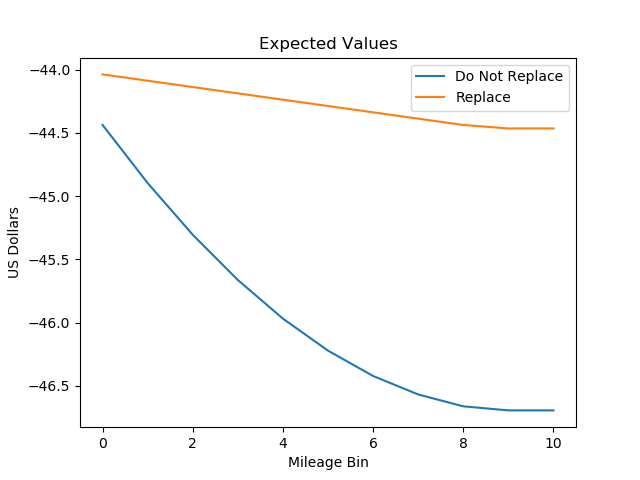
\includegraphics[width=1.0\textwidth]{Figure_1}
\end{figure}
\FloatBarrier

\subsection{Graphs of Choice Probability}

\begin{figure}[h]
  \centering
    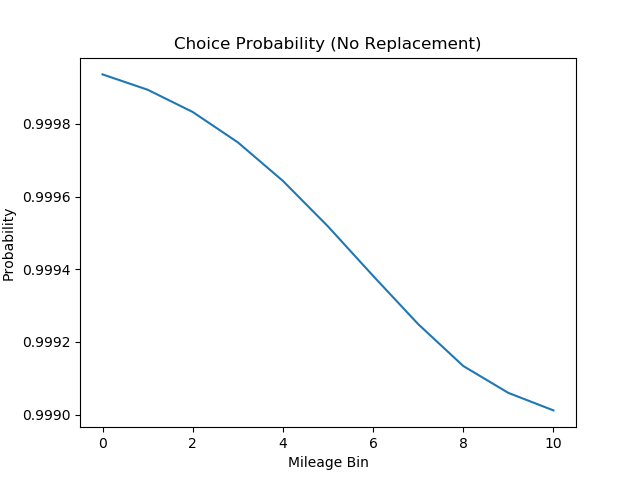
\includegraphics[width=1.0\textwidth]{Figure_2}
\end{figure}
\FloatBarrier

\begin{figure}[h]
  \centering
    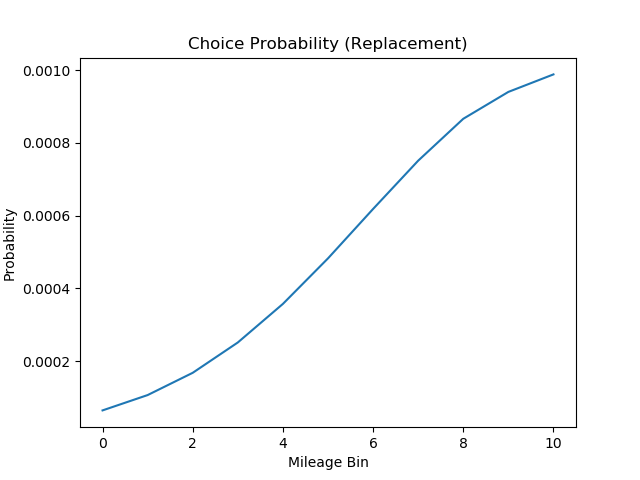
\includegraphics[width=1.0\textwidth]{Figure_3}
\end{figure}
\FloatBarrier

\subsection{Summary Statistics of Simulated Dataset}

Using a seed of $23061994$, I obtain my simulated dataset of state variables $\{ x_t, i_t, \epsilon_t \}$.

% Code Snippet
\begin{lstlisting}
Summary Statistics of State Variable x[t] across [100] Buses
Mean: 4.73287
Std:  3.2951709459601637
Max:  10.0
Min:  0.0

[Epsilon(0)]
Mean: -0.0009730448585669649
Max: 8.06320490171678
Min: -2.4312376822875166

[Epsilon(1)]
Mean: 0.08335043407806184
Max: 7.379166140483501
Min: -2.6733304185053752
\end{lstlisting}

\newpage

\section{Question 2}

\subsection{Estimation of Parameters using Nested Fixed Point Algorithm}

Initial step is to estimate $\theta_3$ as was done below.

\begin{lstlisting}
theta3=[[ 0.00000000e+00 -3.57913930e+08  3.57913931e+08]
 [ 0.00000000e+00 -3.61493080e+08  3.61493081e+08]
 [ 0.00000000e+00 -3.61493080e+08  3.61493081e+08]]
\end{lstlisting}

\subsection{Counterfactual}

Counterfactually, a higher replacement cost and lower maintenance cost would prolong HZ's decision to remain in the state where he avoids replacement contingent on past states of mileage before optimal stopping is reached.

\begin{figure}[h]
  \centering
    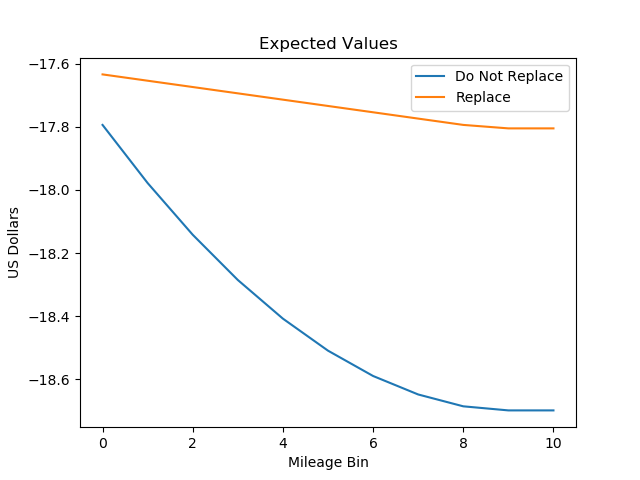
\includegraphics[width=1.0\textwidth]{Figure_4}
\end{figure}
\FloatBarrier

\newpage

\section{Code}

\subsection{Output}

% Code Snippet
\begin{lstlisting}
 RESTART: C:\Users\Dell\Documents\Graduate - Economics\Empirical Industrial Organisation I\
  pset3_working\pset3_SMSajidAlSanai.py 

Question 1:

cost_replacement=10
cost_maintenance=0.05
beta=0.99
theta3=[0.3 0.5 0.2]

Transition Probability Matrix (n x n)
[[0.3 0.5 0.2 0.  0.  0.  0.  0.  0.  0.  0. ]
 [0.  0.3 0.5 0.2 0.  0.  0.  0.  0.  0.  0. ]
 [0.  0.  0.3 0.5 0.2 0.  0.  0.  0.  0.  0. ]
 [0.  0.  0.  0.3 0.5 0.2 0.  0.  0.  0.  0. ]
 [0.  0.  0.  0.  0.3 0.5 0.2 0.  0.  0.  0. ]
 [0.  0.  0.  0.  0.  0.3 0.5 0.2 0.  0.  0. ]
 [0.  0.  0.  0.  0.  0.  0.3 0.5 0.2 0.  0. ]
 [0.  0.  0.  0.  0.  0.  0.  0.3 0.5 0.2 0. ]
 [0.  0.  0.  0.  0.  0.  0.  0.  0.3 0.5 0.2]
 [0.  0.  0.  0.  0.  0.  0.  0.  0.  0.3 0.7]
 [0.  0.  0.  0.  0.  0.  0.  0.  0.  0.  1. ]]

Iteration [843]:
[[-44.43672519 -44.03718872]
 [-44.89646106 -44.0871851 ]
 [-45.30542188 -44.1371813 ]
 [-45.66305082 -44.1871773 ]
 [-45.96880391 -44.23717309]
 [-46.22205426 -44.28716867]
 [-46.4224129  -44.33716403]
 [-46.56858692 -44.38715914]
 [-46.66237856 -44.43715401]
 [-46.69465285 -44.46465107]
 [-46.69465285 -44.46465107]]

Choice Probability (No Replacement)
[0.99993583 0.99989367 0.99983243 0.99974902 0.99964292 0.99951771
 0.99938183 0.99924904 0.99913383 0.99905992 0.99901177]

Choice Probability (Replacement)
[6.41671297e-05 1.06334248e-04 1.67569366e-04 2.50978334e-04
 3.57078639e-04 4.82291458e-04 6.18172606e-04 7.50956047e-04
 8.66173759e-04 9.40078244e-04 9.88229455e-04]

Summary Statistics of State Variable x[t] across [100] Buses
Mean: 4.73287
Std:  3.2951709459601637
Max:  10.0
Min:  0.0

[Epsilon(0)]
Mean: -0.0009730448585669649
Max: 8.06320490171678
Min: -2.4312376822875166

[Epsilon(1)]
Mean: 0.08335043407806184
Max: 7.379166140483501
Min: -2.6733304185053752


Question 2:

theta3=[[ 0.00000000e+00 -3.57913930e+08  3.57913931e+08]
 [ 0.00000000e+00 -3.61493080e+08  3.61493081e+08]
 [ 0.00000000e+00 -3.61493080e+08  3.61493081e+08]]

cost_replacement=20
cost_maintenance=0.02
beta=0.99
theta3=[0.3 0.5 0.2]

Transition Probability Matrix (n x n)
[[0.3 0.5 0.2 0.  0.  0.  0.  0.  0.  0.  0. ]
 [0.  0.3 0.5 0.2 0.  0.  0.  0.  0.  0.  0. ]
 [0.  0.  0.3 0.5 0.2 0.  0.  0.  0.  0.  0. ]
 [0.  0.  0.  0.3 0.5 0.2 0.  0.  0.  0.  0. ]
 [0.  0.  0.  0.  0.3 0.5 0.2 0.  0.  0.  0. ]
 [0.  0.  0.  0.  0.  0.3 0.5 0.2 0.  0.  0. ]
 [0.  0.  0.  0.  0.  0.  0.3 0.5 0.2 0.  0. ]
 [0.  0.  0.  0.  0.  0.  0.  0.3 0.5 0.2 0. ]
 [0.  0.  0.  0.  0.  0.  0.  0.  0.3 0.5 0.2]
 [0.  0.  0.  0.  0.  0.  0.  0.  0.  0.3 0.7]
 [0.  0.  0.  0.  0.  0.  0.  0.  0.  0.  1. ]]

Iteration [752]:
[[-17.79399838 -17.63395976]
 [-17.97813281 -17.65395976]
 [-18.14193814 -17.67395976]
 [-18.28518495 -17.69395976]
 [-18.40764947 -17.71395976]
 [-18.50907658 -17.73395976]
 [-18.58930961 -17.75395976]
 [-18.64783442 -17.77395976]
 [-18.68538008 -17.79395976]
 [-18.69829846 -17.80495976]
 [-18.69829846 -17.80495976]]

***
[EOF] Output Terminates
***
\end{lstlisting}

\subsection{Source}

\lstinputlisting[language=Python]{pset3_SMSajidAlSanai.py}

\end{document}